\section{SMT Model}

\subsection{Decision Variables}

The SMT model is structured in two clearly defined tasks: \textbf{Satisfiability} and \textbf{Optimization}.

\subsubsection{Satisfiability}

Decision variables for this task include:
\begin{itemize}
    \item $match\_schedule_{p,w,m} \in \{\text{true}, \text{false}\}$: true if and only if the match pair $m$ is scheduled in period $p$ of week $w$.
    \item $home_{p,w} \in T$: the home team assigned to the match in period $p$ of week $w$.
    \item $away_{p,w} \in T$: the away team assigned to the match in period $p$ of week $w$.
\end{itemize}

\subsubsection{Optimization}

Additional variables for optimizing the home-away balance:
\begin{itemize}
    \item $flip\_slot_{p,w} \in \{\text{true}, \text{false}\}$: true if the home-away designation for the match in period $p$ of week $w$ is flipped.
    \item $homeEff_{p,w},\, awayEff_{p,w} \in T$: effective home and away teams after considering the flip decision.
\end{itemize}

\subsection{Objective Function}

The optimization goal is to minimize the maximum imbalance $k$ between the number of home and away games played by each team throughout the tournament. Formally,

\[
k^* = \min \big\{\, k \mid \forall t \in T : |H_t - A_t| \leq k \big\}
\]

where:

\[
H_t = \sum_{p,w} [\,homeEff_{p,w} = t\,], 
\quad 
A_t = \sum_{p,w} [\,awayEff_{p,w} = t\,].
\]

The effective home-away assignment considers potential flips:

\[
homeEff_{p,w} = \text{ite}(flip\_slot_{p,w},\, away_{p,w},\, home_{p,w}), 
\quad 
awayEff_{p,w} = \text{ite}(flip\_slot_{p,w},\, home_{p,w},\, away_{p,w}).
\]

\subsection{Constraints}

\subsubsection{Unique match assignment per slot}

Each period-week slot must host exactly one match:

\[
\forall p \in P,\, w \in W: 
\sum_{m \in M} match\_schedule_{p,w,m} = 1.
\]

\subsubsection{Each match pair used exactly once per week}

Each pair of teams can only be assigned once each week:

\[
\forall m \in M,\, w \in W: 
\sum_{p \in P} match\_schedule_{p,w,m} = 1.
\]

\subsubsection{Binding team assignments}

If a match is scheduled, the home and away teams must match the predetermined pairs $rb$:

\[
\forall p \in P,\, w \in W: 
\bigvee_{m \in M} \big(
match\_schedule_{p,w,m} \wedge home_{p,w} = rb_{m,w,0} \wedge away_{p,w} = rb_{m,w,1}
\big).
\]

\subsubsection{Every team plays at most twice in the same period}

For each team $t$ and each period $p$, we count how many times $t$ appears either as home or away in that period over all weeks and require that this total does not exceed two:

\[
\forall t \in T,\, p \in P: 
\sum_{w \in W} \sum_{m \in M} 
\big(
[\,rb_{m,w,0} = t \lor rb_{m,w,1} = t\,] \cdot [\,match\_schedule_{p,w,m}\,]
\big) \leq 2.
\]

\subsubsection{Symmetry breaking}

To reduce equivalent permutations of the solutions, fix the initial assignment:

\[
match\_schedule_{0,0,0} = \text{true}.
\]

\subsubsection{Imbalance constraint}

Ensure that the maximum allowed imbalance $k$ is respected:

\[
|H_t - A_t| \leq k.
\]

\subsection{Validation}

\subsubsection{Experimental design}

The SMT model is implemented in Python using SMT-LIB to interface with Z3 and CVC5 solvers. A two-step approach is followed: first, a feasible schedule satisfying all base constraints is found (\textbf{Satisfiability}); then, a binary search is performed in the range $[1,\, \lfloor(N-1)/2\rfloor]$ to find the minimal imbalance $k$ (\textbf{Optimization}). For each tested value of $k$ in the search, a new \texttt{.smt2} file is generated, resulting in approximately $\log_2(N)$ separate files for the optimization phase, while only one \texttt{.smt2} file is needed for the satisfiability phase. Experiments are run with a time limit of 300 seconds to evaluate solver efficiency and scalability for different instance sizes $N$.


\subsubsection{Experimental results}

The experimental results show that Z3 performs significantly better than CVC5 in terms of solving time and scalability. Specifically, Z3 solved instances up to $N=22$ within the time limit, while CVC5 handled only smaller instances and degraded rapidly beyond $N=8$.

\begin{table}[H]
\centering
\small
\begin{tabular}{|c|c|c|}
\toprule
\textbf{N} & \textbf{Z3} & \textbf{CVC5} \\
\midrule
6  & \textbf{0}   & \textbf{0}   \\
8  & \textbf{0}   & \textbf{1}   \\
10 & \textbf{0}   & N/A \\
12 & \textbf{0}   & N/A \\
14 & \textbf{0}   & N/A \\
16 & \textbf{0}   & N/A \\
18 & \textbf{3}   & N/A \\
20 & \textbf{14}  & N/A \\
22 & \textbf{280} & N/A \\
24 & N/A & N/A \\
\bottomrule
\end{tabular}
\caption{SMT solver runtimes (in seconds)}
\label{table:smt-result}
\end{table}

% \begin{figure}[H]
% \centering
% 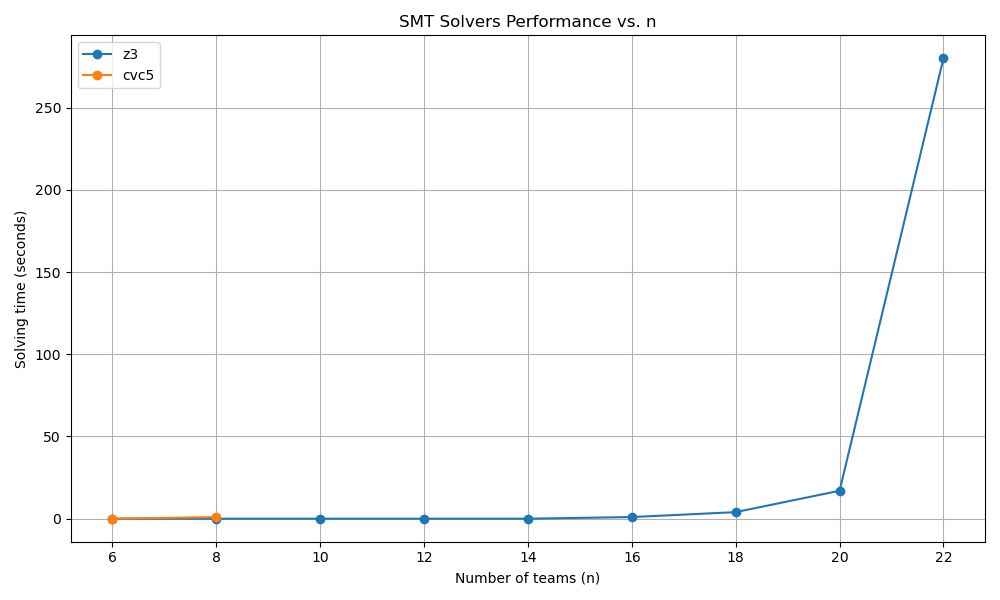
\includegraphics[width=0.8\linewidth]{img/SMT-result.png}
% \caption{SMT solution example}
% \label{fig:smt-result}
% \end{figure}